\documentclass[12pt,a5paper]{book}

\usepackage{phffullpagefigure}

\usepackage{pdfpages}

\usepackage{lipsum}

\sloppy


\begin{document}

\lipsum[1-3]

And see Fig.~\ref{fig:test-1}. Placed using default side/placement, with figcontents command
[FIGCONTENTS].

\begin{fullpagefigure}
  \figcontents{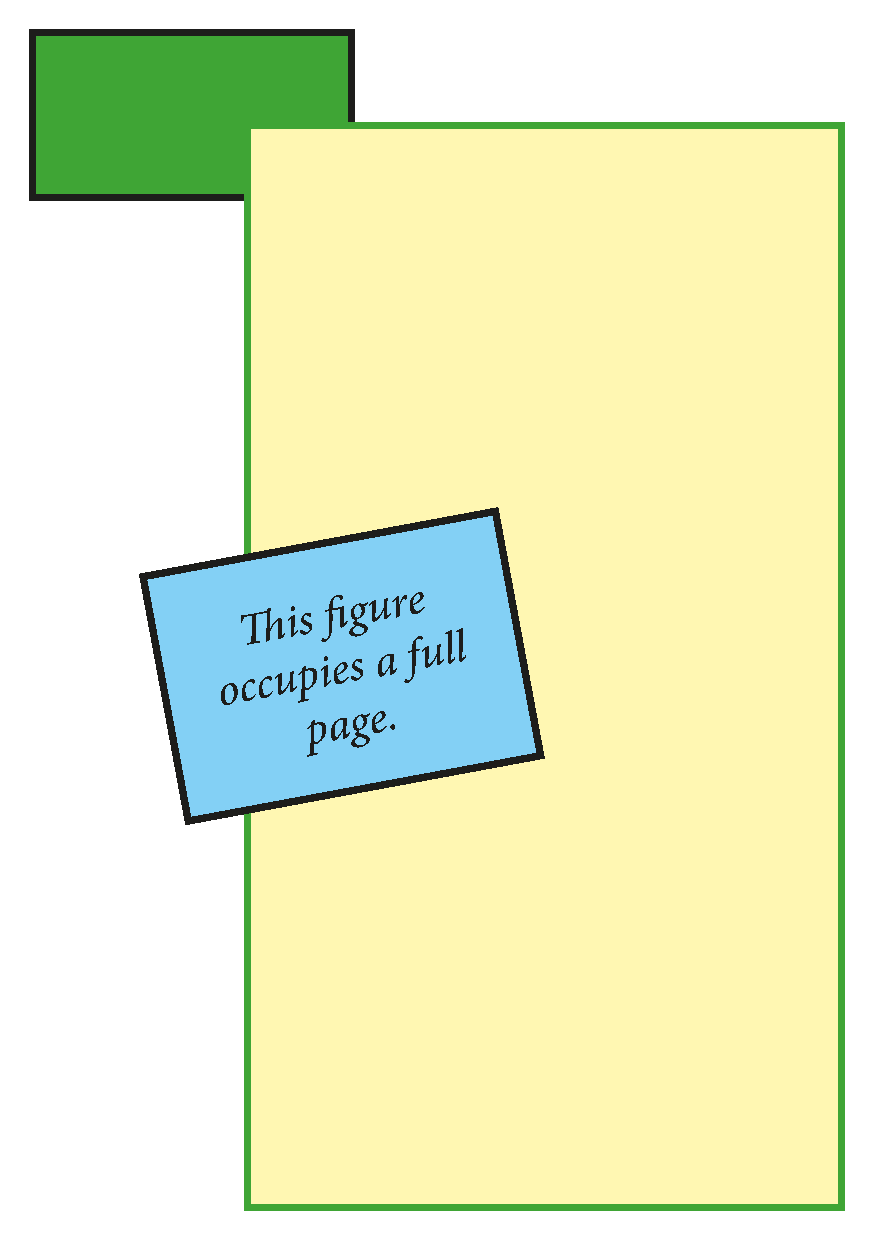
\includepdf{exampleA5fig}}
  \caption{Caption here. This is some text. This is some text. This is some text. This is
    some text. This is some text. This is some text. This is some text. This is some
    text. This is some text. This is some text. This is some text. This is some text. This
    is some text. This is some text. }
  \label{fig:test-1}
\end{fullpagefigure}

\lipsum[5-8]

\cleardoublepage
\lipsum[1-3]

And see Fig.~\ref{fig:test-2}. Placed using default side, with [p] flag [[P],FIGPDF].

\begin{fullpagefigure}[p]
  \figpdf{exampleA5fig}
  \caption{Caption here. This is some text. This is some text. This is some text. This is
    some text. This is some text. This is some text. This is some text. This is some
    text. This is some text. This is some text. This is some text. This is some text. This
    is some text. This is some text. }
  \label{fig:test-2}
\end{fullpagefigure}

\lipsum[5-7]

\cleardoublepage
\lipsum[1-3]

And see Fig.~\ref{fig:test-3}. Placed using default side, with [t] placement [FIGPLACEMENT,FIGPDF].

\begin{fullpagefigure}
  \figpdf{exampleA5fig}
  \figplacement{t}
  \caption{Caption here. This is some text. This is some text. This is some text. This is
    some text. This is some text. This is some text. This is some text. This is some
    text. This is some text. This is some text. This is some text. This is some text. This
    is some text. This is some text. }
  \label{fig:test-3}
\end{fullpagefigure}

\lipsum[5-7]

\cleardoublepage
\lipsum[1-3]

And see Fig.~\ref{fig:test-4}. Placed on an even side page [EVEN,FIGPDF].

\begin{fullpagefigure}
  \figpageside{even}
  \figpdf{exampleA5fig}
  \caption{Caption here. This is some text. This is some text. This is some text. This is
    some text. This is some text. This is some text. This is some text. This is some
    text. This is some text. This is some text. This is some text. This is some text. This
    is some text. This is some text. }
  \label{fig:test-4}
\end{fullpagefigure}

\lipsum[5-7]


\cleardoublepage
\lipsum[1-3]

And see Fig.~\ref{fig:test-5}, which is placed on an odd side page. [ODD,FIGPDF]

\begin{fullpagefigure}
  \figpageside{odd}
  \figpdf{exampleA5fig}
  \caption{Caption here. This is some text. This is some text. This is some text. This is
    some text. This is some text. This is some text. This is some text. This is some
    text. This is some text. This is some text. This is some text. This is some text. This
    is some text. This is some text. }
  \label{fig:test-5}
\end{fullpagefigure}

some small paragraph, before the FLUSH command.

\FlushAllFullPageFigures

A new paragraph, after the flush command.

\lipsum[5-7]


\cleardoublepage
\lipsum[1-3]

And see Fig.~\ref{fig:test-6}. Placed on an even side page [EVEN,FIGPDF].

\begin{fullpagefigure}
  \figpageside{even}
  \figpdf{exampleA5fig}
  \caption{Caption here. This is some text. This is some text. This is some text. This is
    some text. This is some text. This is some text. This is some text. This is some
    text. This is some text. This is some text. This is some text. This is some text. This
    is some text. This is some text. }
  \label{fig:test-6}
\end{fullpagefigure}

\lipsum[5-7]


\cleardoublepage
\lipsum[1-2]

Fine-tune paragraph length:: Nulla malesuada porttitor diam. Donec felis erat, congue non,
volutpat at, tincidunt tristique, libero. Vivamus viverra fermentum felis. Donec nonummy
pellentesque ante. Phasellus adipiscing semper elit. Proin fermentum massa ac quam. Sed
diam turpis, molestie vitae, placerat a, molestie nec, leo. Maecenas lacinia. Nam ipsum
ligula, eleifend at, accumsan nec, suscipit a, ipsum. Morbi blandit ligula feugiat
magna. Nunc eleifend consequat lorem. Sed lacinia nulla vitae enim. Pellentesque tincidunt
purus vel magna. Integer non enim.

And see Fig.~\ref{fig:test-7}. Placed using default side/placement, with max caption
height flag. [FIGPDF,FIGCAPMAXHEIGHT]

\begin{fullpagefigure}
  \figpdf{exampleA5fig}
  \figcapmaxheight{10em}
  \caption{Caption here. This is some text. Short.}
  \label{fig:test-7}
\end{fullpagefigure}

\lipsum[5-11]


\cleardoublepage
\lipsum[1-3]

{\def\FloatBarrier{}
And see Fig.~\ref{fig:test-8}. Placed on an odd side page [ODD,FIGPDF], but within two%
%
\begin{fullpagefigure}
  \figpageside{even}
  \figpdf{exampleA5fig}
  \caption{Caption here. This is some text. This is some text. This is some text. This is
    some text. This is some text. This is some text. This is some text. This is some
    text. This is some text. This is some text. This is some text. This is some text. This
    is some text. This is some text. }
  \label{fig:test-8}
\end{fullpagefigure}%
%
words of this paragraph.}

\lipsum[5-7]

\cleardoublepage
\lipsum[1-3]

\begin{fullpagefigure}
  \figpageside{even}
  \figpdf{exampleA5fig}
  \caption{Caption here. This is some text. This is some text. This is some text. This is
    some text. This is some text. This is some text. This is some text. This is some
    text. This is some text. This is some text. This is some text. This is some text. This
    is some text. This is some text. }
  \label{fig:test-9}
\end{fullpagefigure}
And see Fig.~\ref{fig:test-9}. Placed on an even side page [EVEN,FIGPDF], but at the
beginning of this paragraph.

\lipsum[5-7]


\cleardoublepage
\lipsum[1-3]

\begin{fullpagefigure}
  \figpageside{odd}
  \figpdf[scale=0.25]{exampleA5fig}
  \caption{First caption.}
  \label{fig:test-10}
\end{fullpagefigure}
And see Fig.~\ref{fig:test-10}. Placed on an odd side page [ODD,FIGPDF].
And also see Fig.~\ref{fig:test-11}.  These are several full-page figures requested at
once, with different flags/settings!
\begin{fullpagefigure}
  \figpageside{even}
  \figpdf{exampleA5fig}
  \caption{SECOND CAPTION.}
  \label{fig:test-11}
\end{fullpagefigure}
And also another Fig.~\ref{fig:test-12}!!  These are several full-page figures requested at
once, with different flags/settings!
\begin{fullpagefigure}
  \figpageside{even}
  \figpdf[scale=0.5]{exampleA5fig}
  \caption{3rd 3rd 3rd 3rd 3rd 3rd 3rd 3rd CAPTION.}
  \label{fig:test-12}
\end{fullpagefigure}

\lipsum[5-20]



\end{document}
